\documentclass[12pt,utf8,notheorems,compress,t]{beamer}
\usepackage{etex}

\usepackage{pgfpages}

\usepackage[english]{babel}

\usepackage{ragged2e}
\usepackage{pifont}
\usepackage{accents}
\usepackage{graphbox}
\newcommand{\cmark}{\ding{51}}
\newcommand{\xmark}{\ding{55}}
\DeclareSymbolFont{extraup}{U}{zavm}{m}{n}
\DeclareMathSymbol{\varheart}{\mathalpha}{extraup}{86}

\graphicspath{{images/}}

\usepackage[protrusion=true,expansion=true]{microtype}

\setlength\parskip{\medskipamount}
\setlength\parindent{0pt}

\useinnertheme[shadow=true]{rounded}
\setbeamerfont{block title}{size={}}

\useinnertheme{rectangles}

\usecolortheme{orchid}
\usecolortheme{seahorse}
\definecolor{mypurple}{RGB}{150,0,255}
\setbeamercolor{structure}{fg=mypurple}
\definecolor{myred}{RGB}{150,0,0}
\setbeamercolor*{title}{bg=myred,fg=white}
\setbeamercolor*{titlelike}{bg=myred,fg=white}
\setbeamercolor{frame}{bg=black}

\usefonttheme{serif}
\usepackage[T1]{fontenc}
\usepackage{libertine}

% lifted from https://arxiv.org/abs/1506.08870
\DeclareFontFamily{U}{min}{}
\DeclareFontShape{U}{min}{m}{n}{<-> udmj30}{}
\newcommand\yon{\!\text{\usefont{U}{min}{m}{n}\symbol{'210}}\!}

\setbeamertemplate{headline}{%
  \begin{beamercolorbox}[wd=\paperwidth,ht=2.25ex]{}%
    \insertsectionnavigationhorizontal{\paperwidth}{}{}%
  \end{beamercolorbox}%
  \vskip0pt%
}

\setbeamertemplate{frametitle}{%
  \vskip0.4em%
  \leavevmode%
  \begin{beamercolorbox}[dp=1ex,center]{}%
  %   \usebeamercolor[fg]{item}{\textbf{{\Large \insertframetitle}}}
    \begin{tikzpicture}
      \def\R{8pt}
      \node (title) {\hil{\large\insertframetitle}};
      \begin{pgfonlayer}{background}
        \draw[decoration={bumps,segment length=8pt}, decorate, very thick, draw=mypurple]
          ($(title.south west) + (\R, 0)$) arc(270:180:\R) --
          ($(title.north west) + (0, -\R)$) arc(180:90:\R) --
          ($(title.north east) + (-\R, 0)$) arc(90:0:\R) --
          ($(title.south east) + (0, \R)$) arc(0:-90:\R) --
          cycle;
      \end{pgfonlayer}
    \end{tikzpicture}
  \end{beamercolorbox}%
  \vskip-0.6em%
}

\setbeamertemplate{navigation symbols}{}

\newcommand{\insertframeextra}{}
\setbeamertemplate{footline}{}


\newcommand{\hil}[1]{{\usebeamercolor[fg]{item}{\textbf{#1}}}}
\newcommand{\bad}[1]{\textcolor{red!90}{\textnormal{#1}}}

\begin{document}

\begin{frame}
  \centering
  \vspace*{-0.3em}
  
\includegraphics[width=0.25\textwidth]{hen}
  \\[-0.3em]
  \huge
  \hil{Agda}, \mbox{a
  \textit{beaut$\accentset{\,\,
\includegraphics[width=0.3em]{butterfly}}{\text{\textit{\i}}}$ful} proof assistant}

  \tiny
  second part of the course \textsc{teoria dei tipi} \textbullet{} begin April
  29th, 2020 \textbullet{} by Ingo Blechschmidt

  \normalsize
  \raggedright
  \bigskip

  \begin{columns}
    \begin{column}{0.47\textwidth}
      Agda is \ldots
      \begin{enumerate}
        \item a programming language
        \item a \hil{proof language}
        \item<3-> somewhat hard to learn on one's own
        \item<3-> \hil{fun and easy} to learn as part of a course
      \end{enumerate}
    \end{column}

    \begin{column}[t]{0.61\textwidth}
      \only<1>{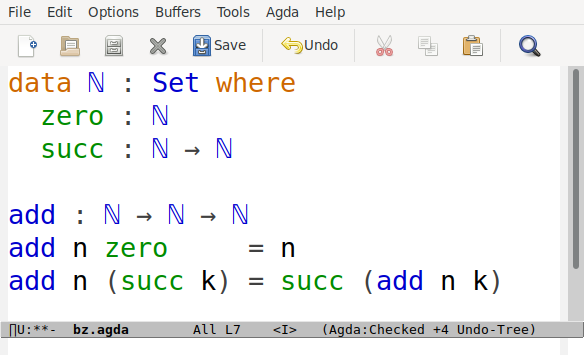
\includegraphics[width=1.0\textwidth,align=t]{agda-example}}
      \only<2->{
        With Agda you can \ldots
        \begin{enumerate}
          \item ensure \hil{correctness} of proofs
          \item \mbox{\hil{practically explore} type theory}
          \item appreciate mathematics from a new point of view
        \end{enumerate}

        \bigskip
        \centering\hil{``proving $=$ programming''}
      }
    \end{column}
  \end{columns}
\end{frame}

\end{document}

addictive

do not learn Agda!


Hello! I'm Ingo Blechschmidt, and I'm here to tell you about what's probably
the single coolest thing I've learned in the last couple years. I'm here to
tell you about Agda, a system put forward by Catarina Coquand in 1999.

First and foremost, Agda is an ordinary programming language. You can write
computer programs in Agda.

But, much more to the point, Agda is also a proof language. You can write
mathematical proofs in Agda, and Agda will check their correctness.
Over the years, using Agda or similar systems, substantial errors and gaps in
published mathematical proofs have been found.

Agda is based on dependent type theory which is introduced in the first part of
the course by professor Maietti. Using Agda, you can actually play with
type theory in the computer, and unlike your pen or your paper, Agda will
always give you immediate feedback.

% There is only one catch. Namely, Agda is somewhat hard to learn on one's own.
% Sometimes, error messages are cryptic and documentation is sparse. Normally,
% this would be a reason to worry. But in this case, you don't need to worry!

We will learn Agda in a series of practical sessions. It will be easy and fun!

If you are a computer scientist, learning Agda will help you understand type
theory and architect correct programs, programs which will not go wrong.

And if you are a mathematician, by learning Agda you will appreciate mathematics
from a new point of view, enjoying proofs from an angle you haven't yet looked at.

Please feel invited. Questions will always be welcome. We will do this together.
Agda is pure elegance, and I'm sure you will enjoy it.
